\section{Keplerian Hohmann Transfer}
Since the orbits of Earth and Mars are assumed to be circular in this investigation, the lowest
maneuver cost transfer between the two bodies using Keplerian dynamics is a Hohmann transfer, shown
in \cref{fig:Hohmann}. However, this only applies if the orbits are coplanar. Hence, a plane change
maneuver must be introduced to account for the difference in the orbital planes. These inclination
change maneuvers are cheapest at apoapsis, so this is achieved by including the plane change in the
maneuver cost of the second Hohmann burn ($\Delta v_{2}$ in \cref{fig:Hohmann}) to form a modified
Hohmann transfer that serves as the baseline $\Delta v$ cost for direct transfers between Earth and
Mars.

\begin{figure}[ht]
    \centering
    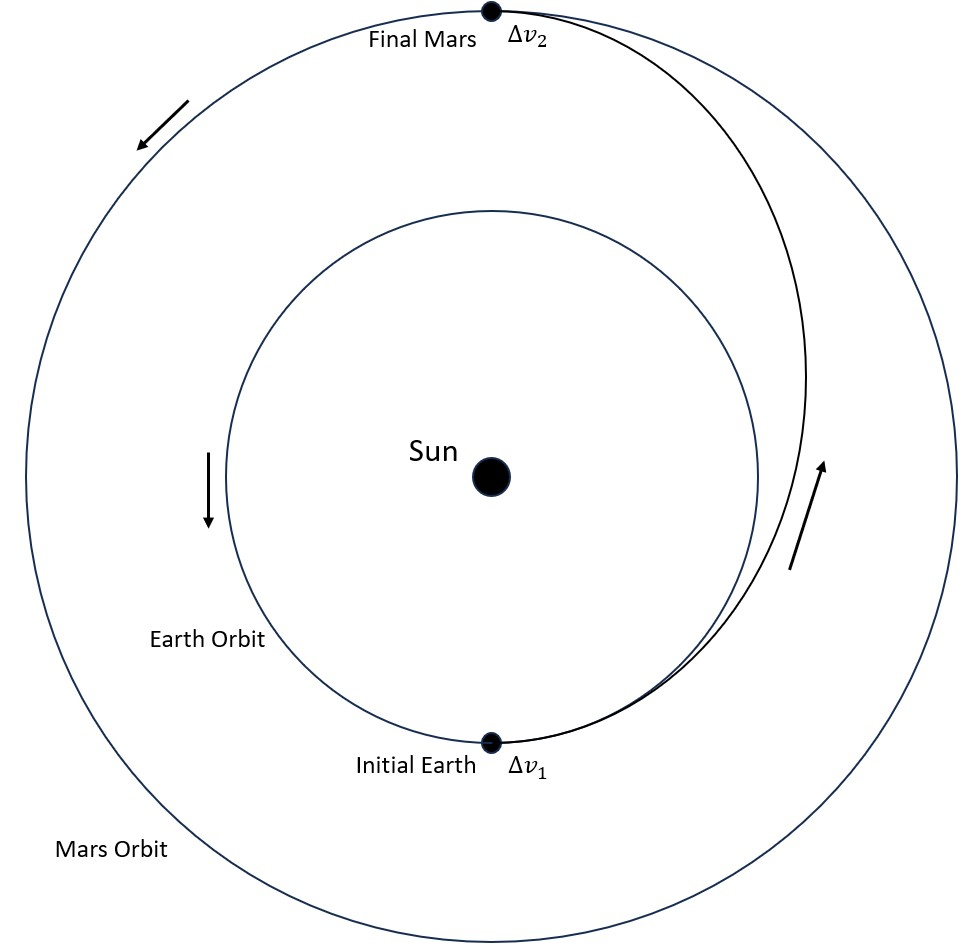
\includegraphics[width=0.5\textwidth]{figures/Hohmann.jpg}
    \caption{Hohmann transfer between Earth and Mars.}
    \label{fig:Hohmann}
\end{figure}


